\documentclass{article}
\usepackage[preprint]{neurips_2025}
\usepackage[utf8]{inputenc}
\usepackage[T1]{fontenc}
\usepackage{amsmath,amssymb,booktabs,graphicx,microtype,array}
\usepackage[hidelinks]{hyperref}
\usepackage{url}
\newcommand{\Sys}{\mathcal{S}}
\newcommand{\Lab}{\textsc{Science Utopia Lab}}
\title{Objective-Conditioned Design of Scientific Institutions}
\author{Science Utopia Lab\\Working research draft, November 7, 2026\\Not submitted; authorship to be finalized}

\begin{document}
\maketitle
\begin{abstract}
Which scientific system is selected when the organizing objective changes?
We treat institutions as executable programs and process graphs inside a
persistent researcher ecosystem. Search changes the organizing system, not
researcher-model weights or the declared objective. Parameters, algorithms,
mechanisms and wiring are composable design freedoms, separate from the
optimization method; whole-world differentiation is unnecessary. We implement
durable propose--execute--measure--revise search, separating technical validity,
loss and outside evaluation. A same-source development comparison contrasts
adaptive feedback with technical-only proposals for two objectives. Of eight
candidates, four complete and four fail during execution. An initial
technical-only all-accept proposal improves both losses, but no measured
second-generation gain or feedback advantage is observed. A subsequent
eight-rule control study completes every world and numerically recovers those
proxy scores with hand-written all-accept rules; removing review also ties the
throughput minimum without review-backed score. Thus weak-seed improvement
alone is insufficient evidence of effective invention. A fixed protocol next
compares numeric, code and structural freedom with selection-before-evaluation;
its outcomes are not yet reported. These pilots establish neither optimizer
superiority, recursive improvement nor real scientific-policy benefit.
\end{abstract}

\section{Introduction}
Scientific institutions coordinate information, resources, evaluation, and
opportunities. Changing one rule may alter the population and evidence that
subsequent rules encounter. A scientific ecosystem is consequently a natural
object of system design, rather than merely a collection of independent tasks.
ScienceUtopia provides a persistent, literature-grounded researcher world for
studying such feedback through institutional interventions
\citep{jin2026scienceutopia}. Our question is different: given an explicit
objective, which organizing system does a search process discover, and why?

The distinction is between \emph{analyzing a specified intervention} and
\emph{searching the intervention's executable definition}. A reviewer-assignment
rule is one possible mechanism, not a required centerpiece. Evaluation,
publication, funding, governance, information exchange, and their presence or
absence are all potential design decisions. The original researcher world is
a contained instance, not a ceiling on future expressiveness or a reason to
replace it with a simpler numerical surrogate.

\begin{figure}[t]
\centering
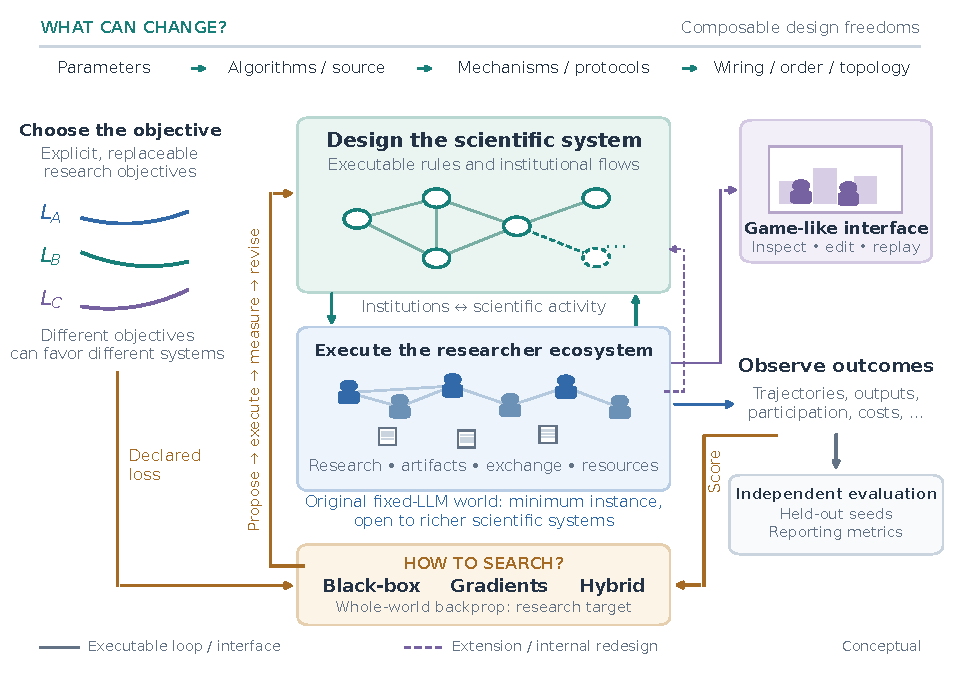
\includegraphics[width=\linewidth]{figures/program-concept/science-system-design-program.pdf}
\caption{\textbf{The research program: scientific systems as design objects.}
Parameter values, executable algorithms, mechanisms, and wiring/processes are
composable freedoms. The objective and search method are separate axes. The
figure is conceptual, not empirical data or a completion map. Full-world
backpropagation and recursive improvement are optional research directions,
not established properties of the development comparison.}
\label{fig:program}
\end{figure}

This problem does not become new merely because an LLM writes code. Prior work
already evolves executable mechanisms against evaluation functions
\citep{liu2025mechanism}, uses past solutions and values in LLM optimization
\citep{yang2024opro}, and combines discrete LLM search with differentiable
continuous optimization \citep{ma2024sga}. The intended contribution is an
executable scientific-system design problem and evidence about how objectives,
design freedom, and search change the resulting institutions. Establishing that
contribution requires matched comparisons and mechanistic findings, not a count
of implemented interfaces or debug iterations.

\section{Problem and design space}
\label{sec:problem}
Let $S\in\Sys$ be an executable scientific-system specification, $W$ fixed
researcher-model weights, $D$ a fixed literature corpus, and $\xi$ the
stochastic inputs of a world. A persistent trajectory is
$\tau\sim P(\cdot\mid S,W,D,\xi)$; researcher responses remain adaptive to
their inputs even though $W$ is fixed. An evaluator extracts measurements
$m=M(\tau)$. For a declared objective $\lambda$, the research target is
\begin{equation}
  \min_{S\in\Sys}\ J_\lambda(S)
  =\mathbb{E}_{\xi,\tau}\left[\ell_\lambda(M(\tau))\right].
  \label{eq:target}
\end{equation}
A finite pilot observes losses, not the global minimum or an exact expectation.
Changing $\lambda$ changes the optimization problem; search changes $S$ rather
than silently editing $\ell_\lambda$ to favor an observed candidate.

\paragraph{Four composable freedoms.}
\emph{Parameters} change numerical settings within a rule.
\emph{Algorithms} replace executable mappings, state updates, and decisions.
\emph{Mechanisms} introduce or remove organizing components, messages, and
state. \emph{Wiring and processes} alter who receives which information and
resources, execution order, and declared repetition. These freedoms are not
four mutually exclusive methods or a fixed institution catalogue. The current
implementation exposes typed SystemSpecs, code mechanisms, graph connections,
and native process execution; not every generated specification is valid.

\paragraph{Four distinct evidence objects.}
The optimization loss $\ell_\lambda$ ranks measured candidates.
Technical validity says whether a candidate can be executed and measured under
the declared interface and budget. Outside evaluation records other outcomes
or unused conditions after selection. An optional deployment policy is a
separate normative decision. Fairness, novelty, or merit is not introduced as a
hidden optimization veto. A technical failure has a null loss, not an invented
large numerical penalty. A proxy optimum is not a universal definition of good
science, nor a recommendation to deploy the resulting institution.

\section{Executable search in the researcher world}
\label{sec:method}
\paragraph{One world, interchangeable proposal methods.}
A durable controller records a request, receives a complete proposed design,
compiles its literal source/graph transaction, executes it in the native
researcher world, measures the outcome, and supplies permitted feedback to the
next request. Proposals may use black-box search or an LLM designer whose
weights also remain fixed. Generated Python executes in the existing isolated
runtime, not on the host. The host does not repair authored scientific rules,
invent missing source, infer a missing finish, or replace a failed candidate
with the baseline. The raw definition and all consumed attempts remain visible.

\paragraph{Gradients are an option, not a world simplification.}
For an explicitly parameterized design distribution $q_\theta$ with complete,
integrable losses and the usual support/differentiation conditions, a
likelihood-ratio identity is
\begin{equation}
 \nabla_\theta\mathbb{E}_{S\sim q_\theta}[\ell(S)]
 =\mathbb{E}_{S\sim q_\theta}[(\ell(S)-b)\nabla_\theta\log q_\theta(S)].
 \label{eq:lr}
\end{equation}
This uses existing estimation ideas \citep{parmas2021unified}; it does not
differentiate arbitrary source code or the fixed LLM. The implementation's
conditional discrete/continuous vocabulary and control variates have explicit
scope. Unknown LLM source-generation probabilities are not differentiated.
Technical failures remain null and prevent score updates for that batch; we
do not claim an unconditional unbiased estimator for arbitrary validity-dependent
search. Whole-world differentiability and gradient superiority are not required
for the black-box comparison below.

\paragraph{No-feedback means no outcome-derived selection channel.}
Removing a scalar score is insufficient if a proposer still receives the best
parent, loss-ranked examples, adaptive strategy weights, or hashes of private
outcomes. Our technical-only control instead uses the fixed initial parent,
cost-independent strategy probabilities, chronological own-authored designs,
and a projected view with ordinal identities. It exposes technical completion
and exception classes, but no losses, measurements, native error strings,
selection labels, or optimizer update reports. The active prompt and every
virtual archive use the same projection; they cannot retrieve the private raw
campaign state. Withholding is labeled explicitly rather than represented as a
technical null. Both groups retain the objective definition.

The adaptive comparison arm receives losses and measurements and selects its
incumbent parent by loss. Its technical exception channel is matched to the
control. This compares the \emph{adaptive feedback package}, including parent
selection, not scalar-score display alone. Technical success itself can be
informative about a world. The boundary is conditional on fixed authored
proposals and technical states, and is not a security sandbox for arbitrary
trusted host callbacks.

\section{Finite same-source development comparison}
\label{sec:experiment}
\paragraph{World and objectives.}
All arms retain the original researcher lifecycle, with five balanced
researchers, two simulated years, seed~42, and the same pinned four-year public
corpus. Researcher inference uses fixed Qwen3-8B weights. The already approved
local 35B designer uses the same bounded authoring profile in every arm. These
are local development conditions, not a reproduction of ScienceUtopia's
reported 32B setup. The shared initial institution is the editable developer
seed \texttt{open\_native\_system}, which already contains code/tensor routing
and an auxiliary cooperative process. It is not the untouched original
quota-based institution. Both objectives were selected after earlier development:
\begin{equation}
  \ell_T=-A,\qquad \ell_E=-Q+0.5R,
\end{equation}
where $A$ counts accepted publication decisions, $Q$ sums the mean original
reviewer overall score for each accepted decision (zero without reviews), and
$R$ counts individual reviews. The exact
versioned LossSpecs and measurement adapters control these definitions. In
particular, $Q$ is not independently verified scientific quality.

\begin{table}[t]
\centering\small
\begin{tabular}{@{}p{.21\linewidth}p{.35\linewidth}p{.35\linewidth}@{}}
\toprule
Property & Adaptive loss feedback & Technical-only proposals\\
\midrule
Objective & Explicit $\ell_T$ or $\ell_E$ & Same objective definition\\
Initial system & Shared fresh native specification & Same specification\\
Future parent & Loss-selected incumbent & Fixed initial system\\
Own history & Designs, outcomes, measured losses & Designs and technical states\\
Exception channel & Class only & Class only\\
Budget & Two candidates per objective & Two candidates per objective\\
Final ranking & Declared loss only & Declared loss only\\
\bottomrule
\end{tabular}
\caption{The information and budget comparison. Historical warm starts are not
used. Generating-arm labels do not veto pooled objective-based selection.}
\label{tab:contract}
\end{table}

\paragraph{Budget and chronology.}
There are eight candidate slots: two objectives, two proposal policies, and
two generations. One separate fresh baseline world provides a common evaluation
reference; its forward measurement vector is scored under both losses but is
not passed to either proposer. The maximum is nine physical worlds and~128
designer authoring calls, with at most~16 actions and~8192 output tokens per
candidate call. Real-backend interface calibration has a separate 40-call cap.
Designer connect/read allowances are $10/900$ seconds per call. No failed slot is
refilled and no successful result is required to close the budget.

Generation~0 has no prior outcome feedback; generation~1 is the first adaptive
comparison. Proposals are separate designer calls, not a shared G0 response
prefix. A shared world seed is not an independent replicate or identical
designer randomness. The driver freezes the source, image, model/backend,
corpus, objective files, initial system, settings, and chronology before
dispatch. A fresh execution-readiness certificate and cold replay precede
generation. Exact-copy equality remains diagnostic rather than a scientific
admission rule; raw received values are preserved.

\paragraph{Current evidence status.}
The comparison is executing at its frozen source. This draft does not report
uncompleted candidates as results or impute their losses. Once the finite budget
closes, original-source replay determines the empirical table and figures;
technical software checks are not substituted for that evidence.


\section{Strong institutional controls}
\label{sec:controls}
The preceding pilot's all-accept proposal raises a basic comparison question:
does automated search add anything beyond obvious hand-written rules?
We therefore evaluate eight developer-defined institutions at a separate frozen
source, retaining the same five-researcher/two-year setting and development
world seed. All eight physical worlds complete. These are baseline evaluations,
not automatic invention, independent environment seeds, or a matched comparison
with the earlier-source pilot.

\begin{figure}[t]
\centering
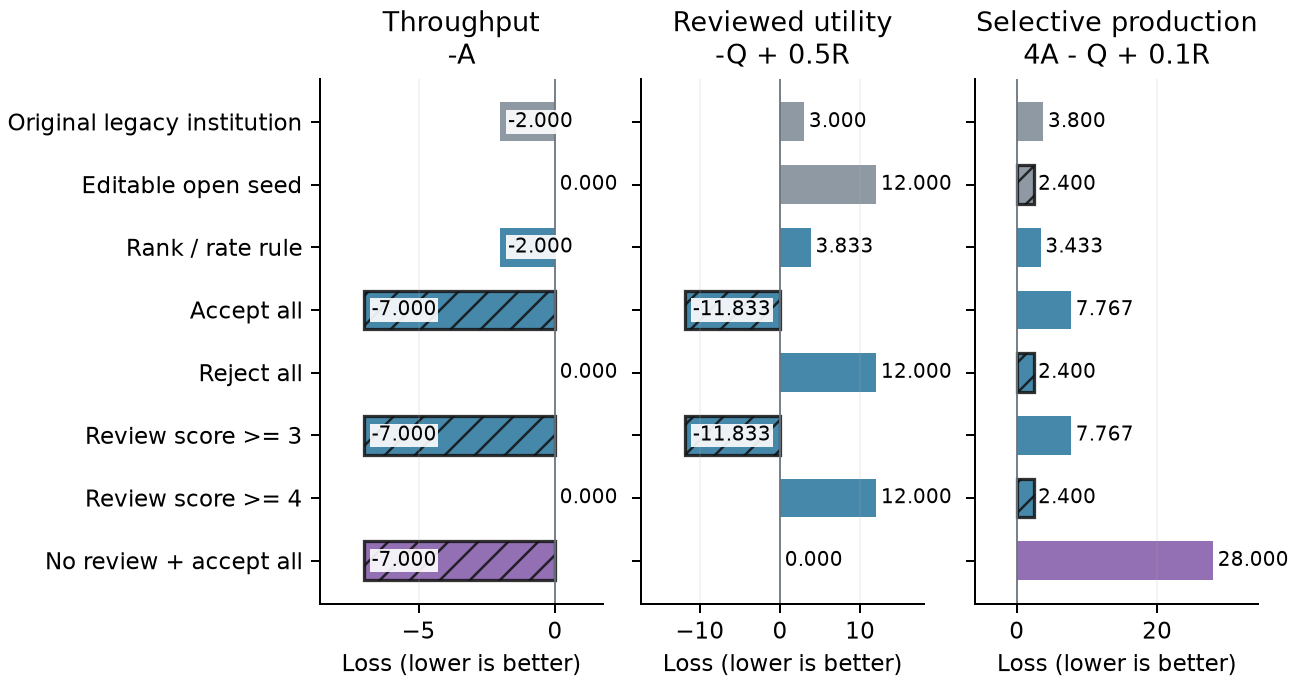
\includegraphics[width=\linewidth]{figures/native-controls-v2-a1-print/strong-controls.png}
\caption{\textbf{Strong-rule controls at one development seed.} All eight
rules complete; smaller values are better. Hatching retains every exact
minimum in each panel. Each panel uses its own scale. $T=-A$ and $E=-Q+0.5R$
are the earlier losses; the explicitly exploratory selective proxy is
$C=4A-Q+0.1R$. Different minima describe different incentives, not scientific
quality or statistical significance. There are no uncertainty intervals from
one environment seed.}
\label{fig:strong-controls}
\end{figure}

The original quota institution produces $A=2,Q=6,R=18$, while the editable
seed produces $A=0,Q=0,R=24$. A rank/rate variant of that seed produces
$A=2,Q=6.667,R=21$. The original and open variants differ in their surrounding
process as well as selection, so this contrast does not isolate a selection
algorithm effect. All-accept and score-threshold~3 both produce
$A=7,Q=22.333,R=21$, giving $T=-7$ and $E=-11.833$. Reject-all and
score-threshold~4 match the seed's $A=0,Q=0,R=24$. Removing review and accepting
all still produces $A=7$, but now $Q=R=0$: it ties the throughput minimum
without any review-backed score. $Q=0$ here follows the declared measurement
convention; it is not evidence of low or high scientific quality.

The developer all-accept control numerically matches the earlier pilot's best
$T/E$ scores, but a cross-source coincidence does not establish method
equivalence. It does establish why weak-seed improvement alone is an inadequate
research endpoint. The eight controls take 37m23s wall time, 726 recorded
scientist responses and 56 institution-code executions, with no designer calls.
Two original-source read-only audits are byte-identical. This closes the
baseline pilot, not the design-freedom study.

\section{Prospectively fixed design-freedom comparison}
\label{sec:prospective}
The next study fixes its objectives, spaces, budgets, chronology and selection
before dispatch. This section is a protocol, \emph{not experimental results}.
Its two primary losses are throughput $T=-A$ and selective production
$C=4A-Q+0.1R$; $E$ remains a cross-score diagnostic. The latter is a declared
trade-off on the native 1--5 review scale, not a normative scientific-value
function. Choosing it after development is exploratory. Its coefficients are
not changed after observing this study's outcomes.

\paragraph{Nested freedoms, separate proposal methods.}
The numeric space permits six explicitly bounded coordinates in the initial
system. The fixed-graph code space adds the three existing Python sources,
including a process delegate, while fixing schemas, ports, nodes, edges and
schedules. The code-and-graph space permits technically valid organizing-system
edits, with the environment seed fixed during development and the original
researcher world, model weights and measurement adapters outside search.
Domains are checked against the original anchor on every proposal; no sequence
of small changes escapes the declared numeric/fixed-graph restrictions.
An out-of-domain literal is retained as a null trial, never projected or repaired.

For each primary objective, we compare LLM proposals in each of the three
domains, a technical-only code-and-graph control, and uniform numeric proposals
without designer calls. Three fresh search histories use controller seeds
42/1031/2063, with four proposals per arm: 120 slots. All development worlds use
world seed 42; three controller histories are not three environment replicates.
Nine fresh reference worlds include the original institution, the editable seed,
and obvious hand rules, including reviewer-free reject-all. No older-source
baseline world is substituted. There are at most 16 charged author actions per
LLM proposal, with no failed-slot refills. Each run requires fresh finite
real-backend calibration. The scientist HTTP caps are 512 per two-year world
and 1024 per four-year world; a cap-exhausted trajectory retains a technical null.

\paragraph{Selection then unused-condition evaluation.}
For each arm/objective, selection pools that arm's three histories plus the
common initial system, retaining all exact ties and choosing the first in a
fixed chronology for physical evaluation. A separate pooled ranking spans all
arms and references without a generating-arm veto. Physical completion and
objective-input availability remain distinct: missing one loss does not erase
other independently measured losses. Selection is hash-frozen before evaluation
on five previously unused world seeds at two years, plus one of those seeds
at four years. Only the declared initial-state seed changes; the policy remains
fixed. Identical policies share physical evaluation explicitly. The maximum is
114 evaluation worlds and 243 worlds including development. Longer and shorter
trajectories at the same seed are not independent samples. All raw values,
missing pairs and costs must be reported before conclusions about design freedom.

\section{What constitutes a research finding?}
\label{sec:analysis}
\paragraph{Objective-conditioned consequences.}
Report all trials and best-so-far paths, a full candidate-by-objective
cross-score matrix, the shared baseline, and all exact ties. Separate own-arm
paths from pooled loss-only selection across generating arms. Cross-scoring
the same checkpoint is a descriptive reuse of one measurement vector, not an
independent replication. Different objectives need not produce different
winners, and a development improvement need not persist on unused conditions.

\paragraph{Mechanisms rather than labels.}
A changed parameter, source fingerprint, or designer explanation is not proof
of implemented behavior. Trace the actual consumer of each edited field,
executed code receipt, changed information delivery, and downstream researcher
inputs/actions. Distinguish source edits that never execute, inert parameters,
and rules that affect outcomes. If an objective rewards publication count or
favorable-review selection, describe the corresponding incentive rather than
renaming it improved scientific quality. Outside evaluation must not silently
become an additional search constraint.

\paragraph{Compute and generalization.}
Count logical slots and physical worlds separately. Report scientist replies,
designer calls, measured tokens and durations, loads, code executions, failures,
and audit costs without adding overlapping wall-time intervals. Equal oracle
budgets do not imply equal total compute. A publication-strength study must
also compare parameter-only, free-code/fixed-graph, and free-graph/process
search under matched conditions, including the unmodified legacy institution
and obvious hand-written rules as stronger controls. After fixing the selection procedure, test
on unused seeds/conditions without feeding them back into search. Researchers
and years within one world are not independent sample units.

\section{Related work and limitations}
\paragraph{Prior methodological building blocks.}
Automated social policy optimization is established, including learned tax
design in simulated economies \citep{zheng2020economist}. AMD-LLM evolves code
mechanisms with a problem-specific fixing process \citep{liu2025mechanism}; our
no-host-repair contract differs, but that alone establishes no performance
advantage. ADAS already searches code-defined agentic workflows using an archive
and evaluation feedback \citep{hu2024adas}. LLM Economist optimizes bounded tax
actions in context over adapting LLM workers \citep{karten2025economist}; frozen
model weights are therefore not a distinctive claim about frozen behavior.
AgentSociety2 supports composable social environments and specification-to-code
generation \citep{piao2026agentsociety2}. Neither executable social research nor
free workflow/code generation is unique to this project.
OPRO already uses evaluated solutions in LLM optimization
\citep{yang2024opro}, and SGA combines LLM discrete search with differentiable
continuous optimization \citep{ma2024sga}. Our proposed contribution must be
supported by scientific-system design comparisons and findings, not by
claiming those generic loops or estimator identities as new.

\paragraph{Scope of this draft.}
The local world is short and small, uses one researcher model and development
seed, and retrieves literature rather than carrying out physical scientific
experiments. Results cannot by themselves validate science-policy objectives
or justify deployment. Two generations cannot demonstrate sample efficiency,
stable autonomous invention, or recursive improvement of the inventor.
Greater API freedom is not evidence that search exploits it effectively.
An executable proposal can also misinterpret the objective's arithmetic;
technical calibration does not establish mathematical task comprehension.
Poor proposals remain in the finite budget rather than being repaired or
replaced by the host. Prospective prompt-display changes require a new source
and calibration instead of silently changing an active comparison.
Conditional gradient support is not a whole-world Jacobian. The English
game-like interface renders the same evidence; it is an artifact/interpretation
aid, not a separate scientific outcome or completed management game.

\section{Conclusion}
The organizing scientific system is a searchable object whose definition can
extend beyond parameter tuning to code, mechanisms, and processes. The research
question is how objectives and design freedom shape the systems discovered and
their consequences. The comparison and reporting boundary make that question
testable without requiring whole-world differentiability or discarding failed
and tied outcomes. The development pilot records a simple initial all-accept
proposal improving both declared proxies, but no measured iterative gain or
feedback superiority. The subsequent strong-rule pilot recovers the earlier
proxy minimum using simple hand rules. The next comparison therefore fixes
freedom ablations and selection before unused-condition evaluation. Those results
and mechanistic evidence are still required; the protocol is not their substitute.
Further freedom ablations, unused-condition evaluation,
and mechanistic evidence are necessary before strong empirical or deployment
claims, and before treating this working draft as a completed conference paper.

\bibliographystyle{plainnat}
\bibliography{references,submission-sources}

\appendix
\section{Reproducibility and evidence boundary}
The finite comparison's original source is
\texttt{2e375c22793210d3496450a99ca96a86f0f7aecc}.
The prospective protocol is retained in the repository's campaign records.
Actual author/native journals, code contexts, response caches, checkpoints,
writer receipts, and exact source/helper hashes remain separate from compact
tables and figures. A read-only auditor reconstructs author tool transitions
and domain measurements, preserves nulls and all candidates, cold-replays the
calibration, and verifies that raw files do not change. Raw caches are not
committed to Git. Test counts and local interface calibration are software
evidence, not additional scientific worlds or proofs of universal reliability.

{\raggedright
The separate eight-rule pilot uses source
\texttt{2aa02c3cb4610cde4797744386da67fe851383b0}; its exact full-audit
content hash is
\texttt{3a344dcbc71c8300d0844696d44b807d3}\allowbreak\texttt{a5ba0eeca14301b1d50c60dd4656ac1}.
The prospective design-freedom study is pinned separately at
\texttt{b6654adefc42223f9ecc7b4e53c043c879230f68}, with an immutable
plan and a pre-dispatch seed-usage inventory. Its future measurements are not
pooled with the completed pilots as if generated under a common source.\par}

The historical long manuscript and development studies remain available as
separate records. Their sources, author provenance, losses, seeds, histories,
and costs are not pooled into this matched comparison. The bundled 2025 style
is used for a readable working draft, not claimed compliance with an unverified
future conference's format, anonymity rules, or submission deadline.
\end{document}
